\documentclass{beamer}
\usepackage[utf8]{inputenc}
\usepackage[russian,english]{babel}
\usepackage{graphicx, epsfig}
\usepackage{amsmath,mathrsfs,amsfonts,amssymb}
\usepackage{subfig}
\usepackage{floatflt}
\usepackage{epic,ecltree}
\usepackage{mathtext}
\usepackage{fancybox}
\usepackage{fancyhdr}
\usepackage{multirow}
\usepackage{enumerate}
\usepackage{epstopdf}
\usepackage{multicol}
\usepackage{algorithm}
\usepackage[noend]{algorithmic}
\def\algorithmicrequire{\textbf{Input:}}
\def\algorithmicensure{\textbf{Output:}}
\usetheme{Singapore}%{Singapore}%{Warsaw}%{Warsaw}%{Darmstadt}
\usecolortheme{default}
\setbeamertemplate{footline}[page number]{}

\newcommand{\bx}{\mathbf{x}}
\newcommand{\by}{\mathbf{y}}
\newcommand{\bw}{\mathbf{w}}
\newcommand{\bY}{\mathbf{Y}}
\newcommand{\bX}{\mathbf{X}}
\newcommand{\bu}{\mathbf{u}}
\newcommand{\bt}{\mathbf{t}}
\newcommand{\bp}{\mathbf{p}}
\newcommand{\bq}{\mathbf{q}}
\newcommand{\bc}{\mathbf{c}}
\newcommand{\bP}{\mathbf{P}}
\newcommand{\bT}{\mathbf{T}}
\newcommand{\bQ}{\mathbf{Q}}
\newcommand{\bC}{\mathbf{C}}
\newcommand{\bE}{\mathbf{E}}
\newcommand{\bF}{\mathbf{F}}
\newcommand{\bU}{\mathbf{U}}
\newcommand{\bW}{\mathbf{W}}
\newcommand{\btheta}{\boldsymbol{\theta}}
\newcommand{\bTheta}{\boldsymbol{\Theta}}
\newcommand{\T}{^{\text{\tiny\sffamily\upshape\mdseries T}}}


\newtheorem{statement}{Statement}

\DeclareMathOperator*{\argmin}{arg\,min}
\DeclareMathOperator*{\argmax}{arg\,max}

%\definecolor{beamer@blendedblue}{RGB}{15,120,80}
%----------------------------------------------------------------------------------------------------------
\title[\hbox to 56mm{  \hfill\insertframenumber\,/\,\inserttotalframenumber}]
{\\ \vspace{1.5cm} Dimensionality reduction for time series decoding and forecasting}
\author[Roman Isachenko]{\\ 
	\vspace{.4cm}
	Roman Isachenko}
\institute[SkolTech]{Moscow Institute of Physics and Technology \\ 
	\vspace{0.1cm}
	Skolkovo Institute of Science and Technology
}
\date{December 25, 2017.}
%--------------------------------------------------------------------------------
\begin{document}
%--------------------------------------------------------------------------------
\begin{frame}
%\thispagestyle{empty}
\titlepage
\end{frame}
%--------------------------------------------------------------------------------
\begin{frame}{Timeline}
		\begin{description}
			\item[September] \footnotesize{quadratic programming approach were investigated, the problem was not formulated properly}
			\vfill
			\item[October] \footnotesize{MMRO-2017 conference, Taganrog,
			"Feature Generation for Physical Activity Classification"
			The paper was prepared and submitted to the journal}
		\vfill
		\item[November] \footnotesize{The research about time series decoding were begun. The new method was proposed.}
		\vfill
		\item[December] \footnotesize{The research was narrowed down, the experiments were conducted, the paper was prepared}
		\end{description}
\end{frame}
%--------------------------------------------------------------------------------
\begin{frame}{Problem Statement}
	Given a dataset $\mathfrak{D}= \left( \bX, \bY \right)$
	\begin{itemize}
		\item $\mathbf{X} \in \mathbb{R}^{m \times n}$ is a design matrix, 
		\item $\mathbf{Y} \in \mathbb{R}^{m \times r}$ is a target matrix. 
	\end{itemize}

	We assume that there is a linear dependence between the objects $\bx \in \mathbb{R}^n$ and the responses $\by \in \mathbb{R}^r$
	\begin{equation*}
	\underset{1 \times r}{\by} = \underset{1 \times n}{\vphantom{\by}\bx} \cdot \underset{n \times r}{\vphantom{\by}\bTheta} + \underset{1 \times r}{\vphantom{\by}\boldsymbol{\varepsilon}}.
	\label{eq::model}
	\end{equation*}
	
	\begin{block}{Error function}
	\begin{equation*}
	S(\bTheta | \mathfrak{D}) = {\left\| \underset{m \times n}{\vphantom{\by}\mathbf{X}} \cdot \underset{n \times r}{\vphantom{\by}\bTheta} - \underset{m \times r}{\vphantom{\by}\mathbf{Y}} \right\| }_2^2 = \sum_{i=1}^m \left\| \underset{1 \times n}{\vphantom{\by}\bx_i} \cdot \underset{n \times r}{\vphantom{\by}\bTheta} - \underset{1 \times r}{\vphantom{\by}\by_i} \right\|_2^2 \rightarrow\min_{\bTheta}.
	\label{eq::error_function}
	\end{equation*}
	\end{block}
	
\end{frame}
%--------------------------------------------------------------------------------
\begin{frame}{Partial Least Squares Regression}
	PLS algorithm finds the matrix $\bT$ in the low-dimensional latent space. The $\bT$ jointly describes the input matrix $\bX$ and the target matrix $\bY$.
	\begin{align*}
	\underset{m \times n}{\vphantom{\bQ}\bX} 
	&= \underset{m \times l}{\vphantom{\bQ}\bT} \cdot \underset{l \times n}{\vphantom{\bQ}\bP^{\T}} + \underset{m \times n}{\vphantom{\bQ}\bF} 
	= \sum_{k=1}^l \underset{m \times 1}{\vphantom{\bp_k^{\T}}\bt_k} \cdot \underset{1 \times n}{\bp_k^{\T}} + \underset{m \times n}{\vphantom{\bp_k^{\T}}\bF},\\
	\underset{m \times r}{\vphantom{\bQ}\bY} 
	&= \underset{m \times l}{\vphantom{\bQ}\bT} \cdot \underset{l \times r}{\bQ^{\T}} + \underset{m \times r}{\vphantom{\bQ}\bE}
	=  \sum_{k=1}^l  \underset{m \times 1}{\vphantom{\bq_k^{\T}}\bt_k} \cdot \underset{1 \times r}{\bq_k^{\T}} +  \underset{m \times r}{\vphantom{\bq_k^{\T}}\bE},
	\end{align*}
\end{frame}
%--------------------------------------------------------------------------------
\begin{frame}{PLS pseudocode}
\begin{figure}
	\begin{flushleft}
	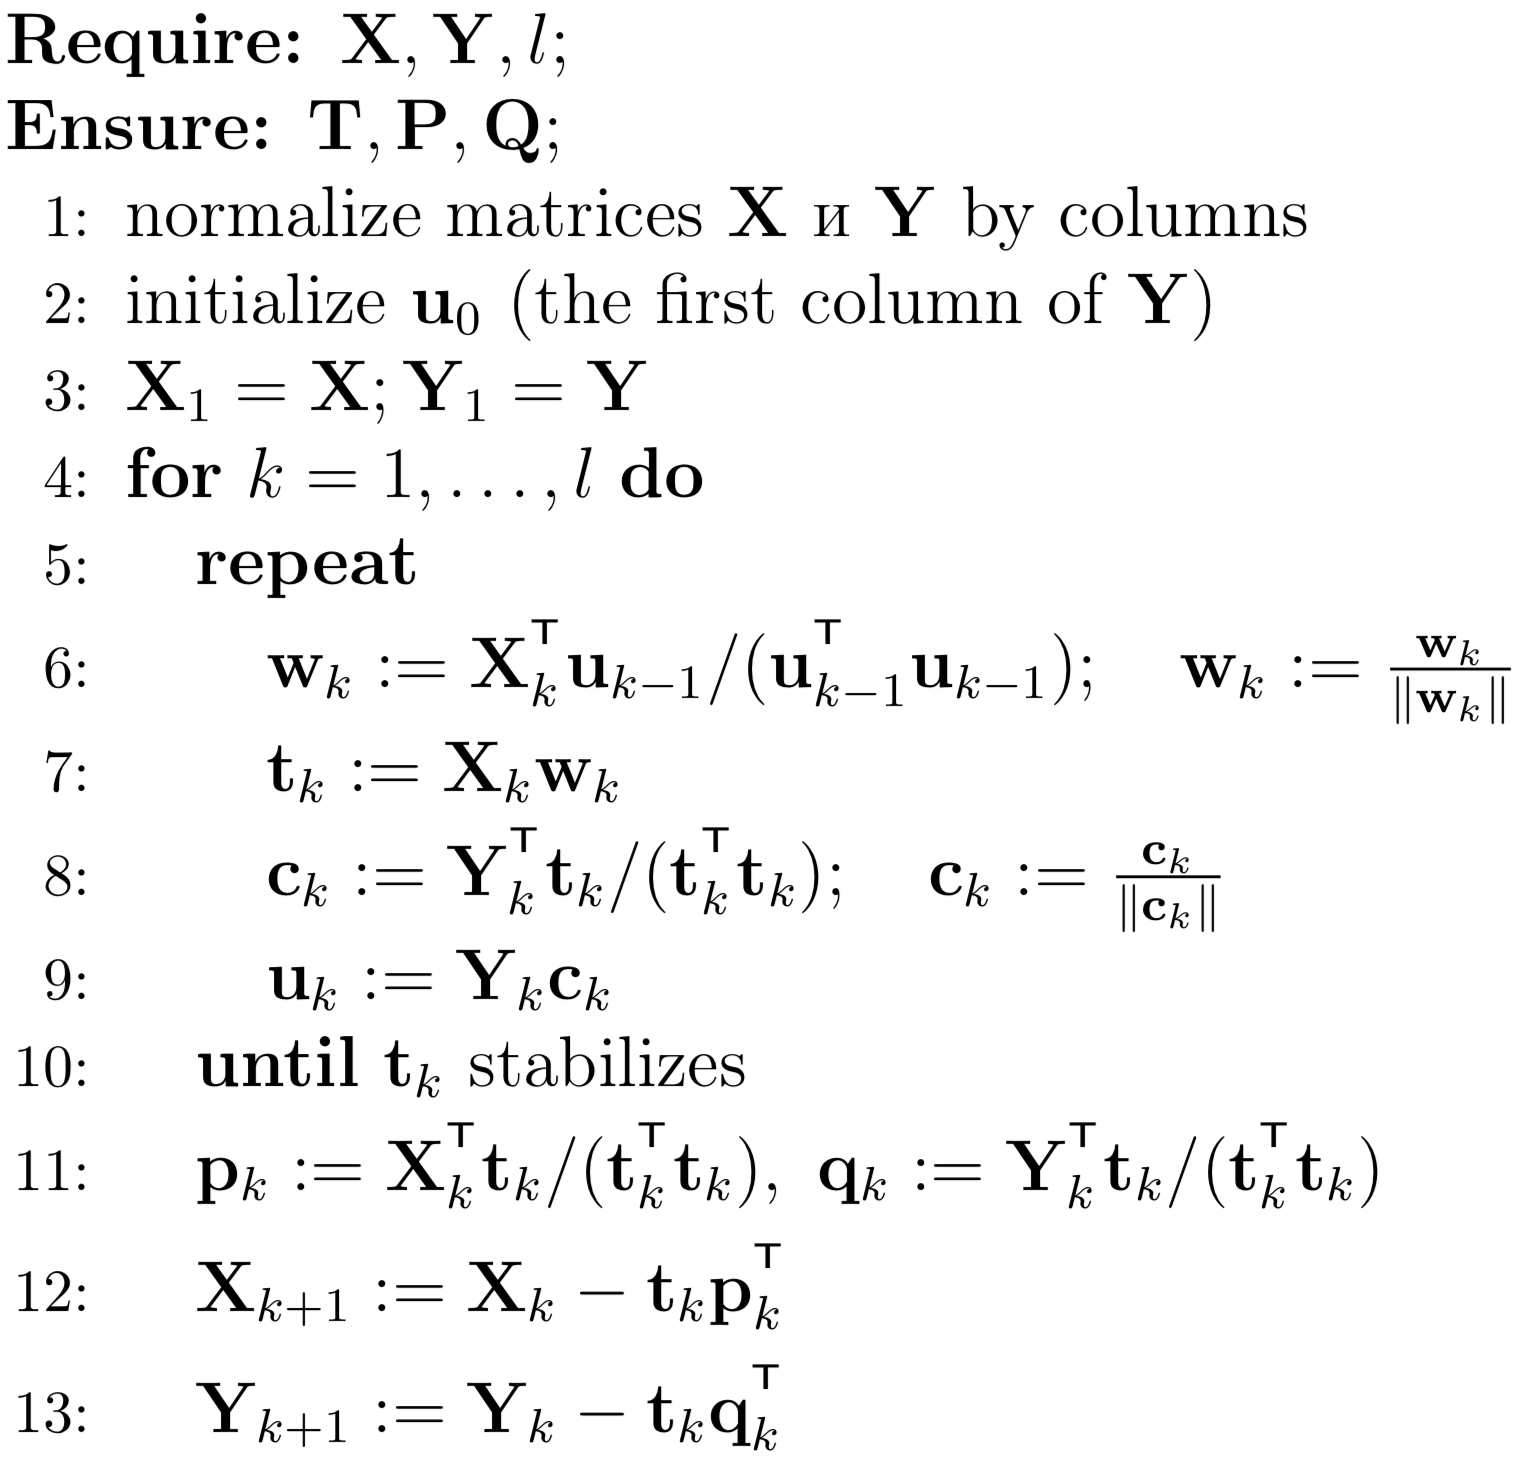
\includegraphics[width=0.7\linewidth]{figs/pls_pseudocode}
\end{flushleft}
\end{figure}
\end{frame}
%--------------------------------------------------------------------------------
\begin{frame}{PLS Example}
\begin{figure}
	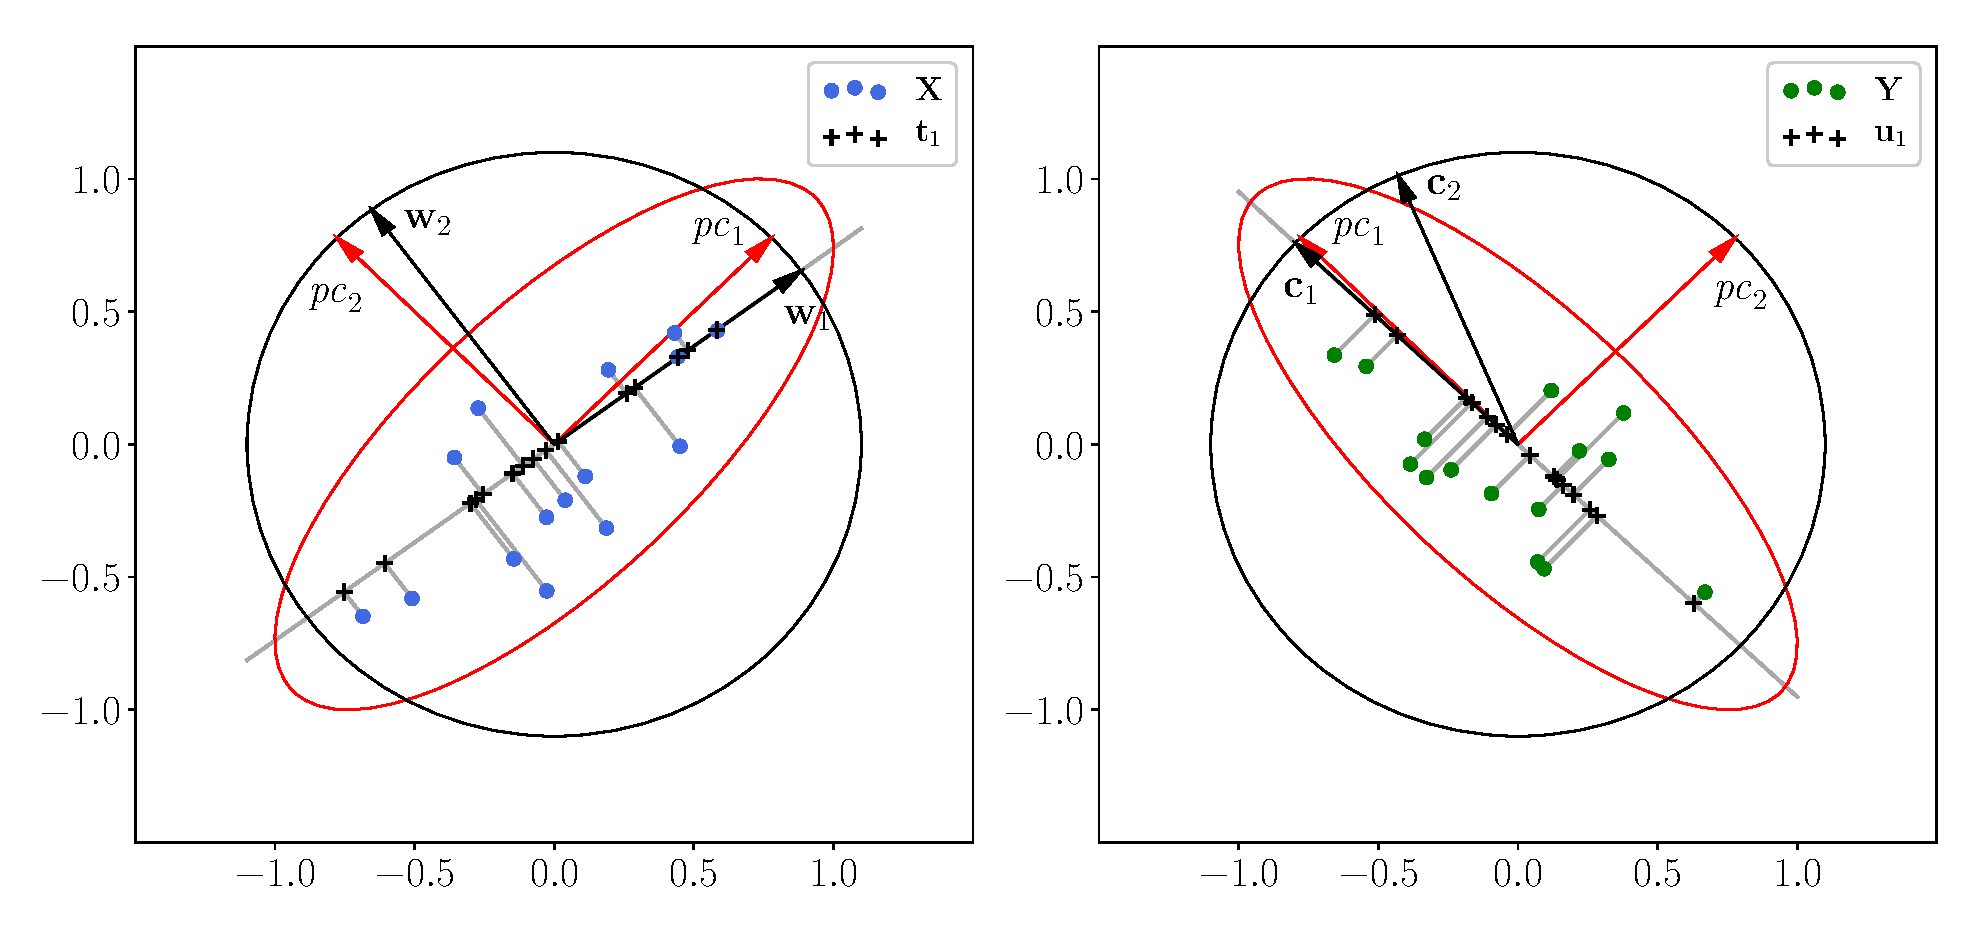
\includegraphics[width=\linewidth]{figs/PLSFigure.eps}
	\caption{The result of the PLS algorithm for the case $n = r = l = 2$.}
\end{figure}
\end{frame}
%--------------------------------------------------------------------------------
\begin{frame}
	\begin{statement}
		The best description of the matrices $\bX$ and $\bY$ taking into account their interrelation is achieved by maximizion the covariance between the vectors $\bt_k$ and $\bu_k$.
	\end{statement}
	\vfill
	\begin{statement}
		The vector $\bw_k$ and $\bc_k$ are eigenvectors of the matrices $\bX_k^{\T} \bY_k \bY_k^{\T} \bX_k$ and $\bY_k^{\T} \bX_k \bX_k^{\T} \bY_k$, corresponding to the maximum eigenvalues.
	\end{statement}
	\vfill
	\begin{statement}
		The update rule for the vectors in steps (6)--(9) of the PLS algorithm corresponds to the maximization of the covariance between the vectors $\bt_k$ and $\bu_k$.
	\end{statement}
	
\end{frame}
%--------------------------------------------------------------------------------
\begin{frame}{PLS solution}

	The linear transformation between objects in the input and latent spaces has the form
	\begin{equation*}
	\bT = \bX \bW^*,
	\label{eq::W*}
	\end{equation*}
	where $\bW^* = \bW (\bP^{\T} \bW)^{-1}$.

	\begin{equation*}
	\bY = \bT \bQ^{\T} + \bE = \bX \bW^* \bQ^{\T} + \bE = \bX \bTheta + \bE.
	\end{equation*}
	The model parameters~\eqref{eq::model} are equal to
	\begin{equation*}
	\bTheta = \bW (\bP^{\T} \bW)^{-1} \bQ^{\T}.
	\label{eq::model_parameters}
	\end{equation*}
	
\end{frame}
%--------------------------------------------------------------------------------
\begin{frame}{Computational experiment}
\begin{minipage}{0.5\textwidth}
	\begin{block}{Datasets}
		\vspace{0.35cm}
		\begin{itemize}
			\item energy consumption
			\item electrocorticogram signals
		\end{itemize}
	\end{block}
\vspace{0.5cm}
\end{minipage}%
\begin{minipage}{0.5\textwidth}
\begin{block}{Autoregressive approach}
	\footnotesize{
	\[
	\mathbf{X} = 
	\begin{pmatrix}
	x_1 & x_2 & \dots & x_n \\
	x_2 & x_3 & \dots & x_{n+1} \\
	\dots & \dots & \dots & \dots \\
	x_{T-n+1} & x_{T-n+2} & \dots & x_T
	\end{pmatrix}.
	\]}
\end{block}
\end{minipage}

\begin{figure}
	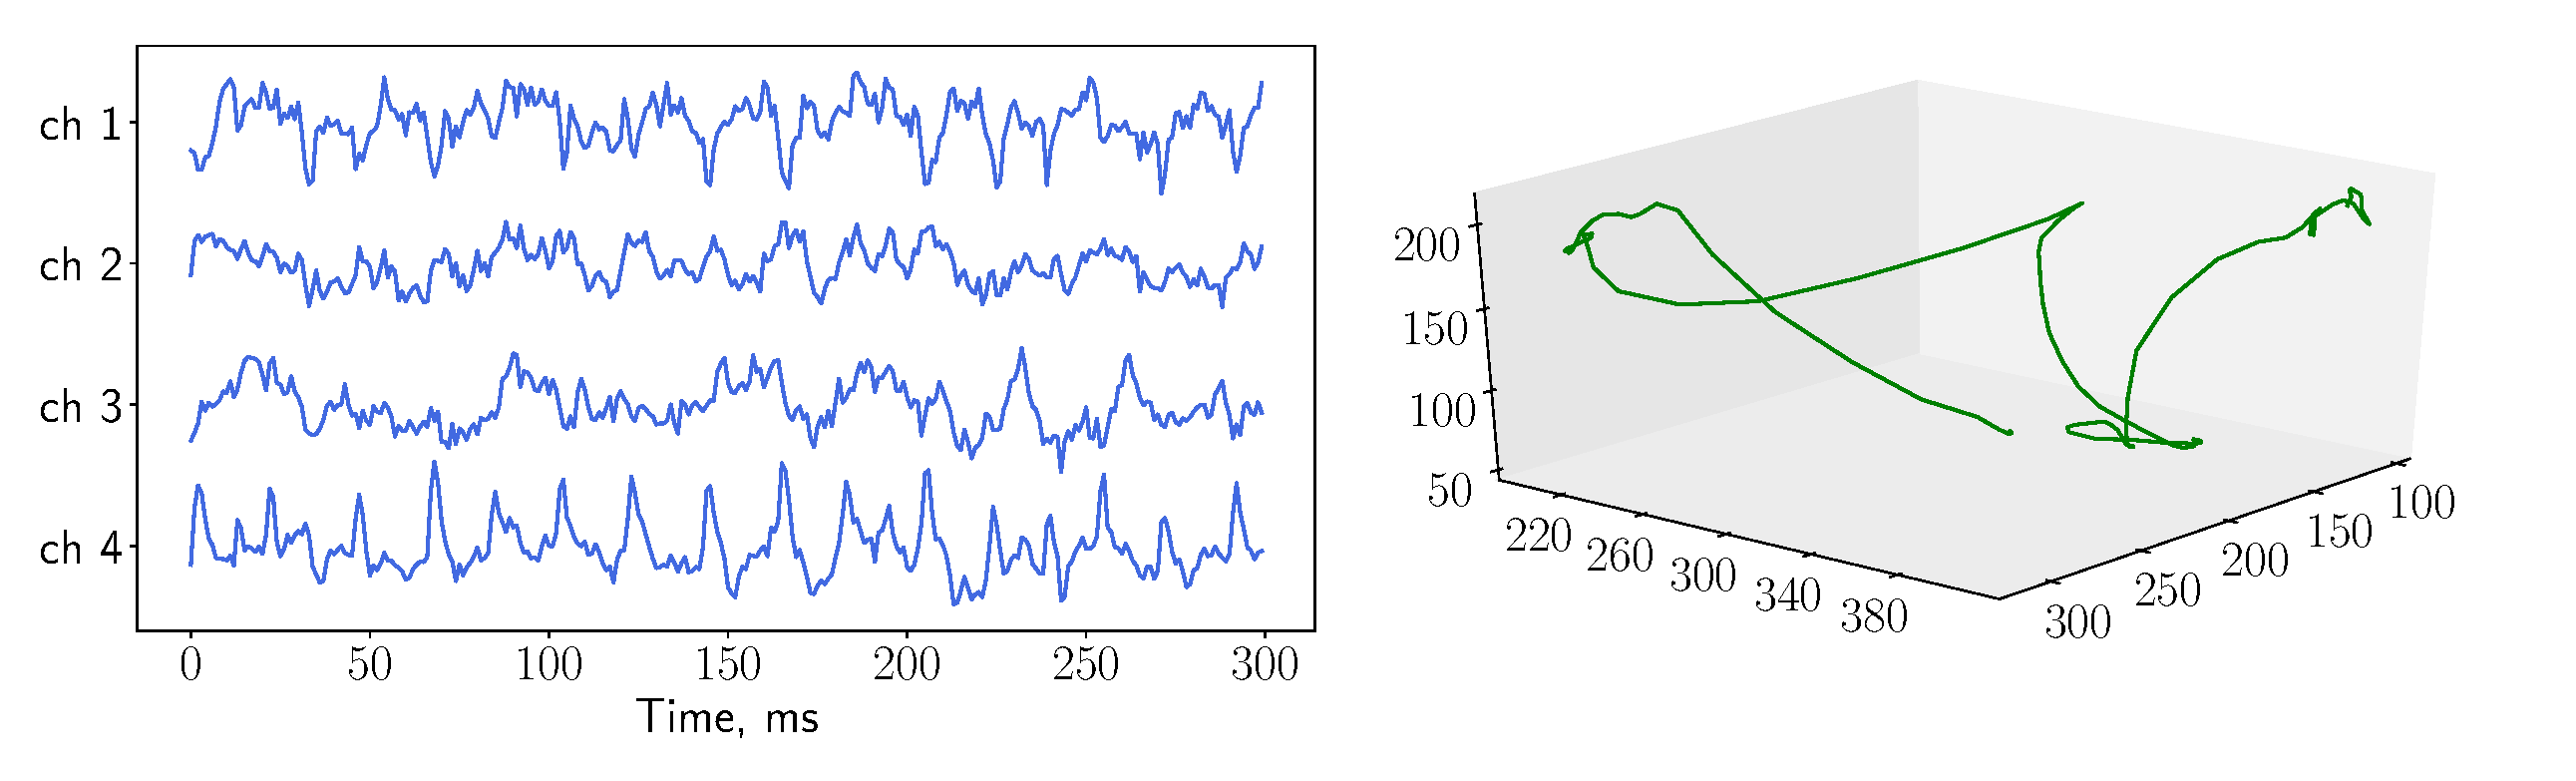
\includegraphics[width=\linewidth]{figs/ecog_data}
\end{figure}
\end{frame}
%--------------------------------------------------------------------------------
\begin{frame}{Computational experiment}
	\begin{figure}
		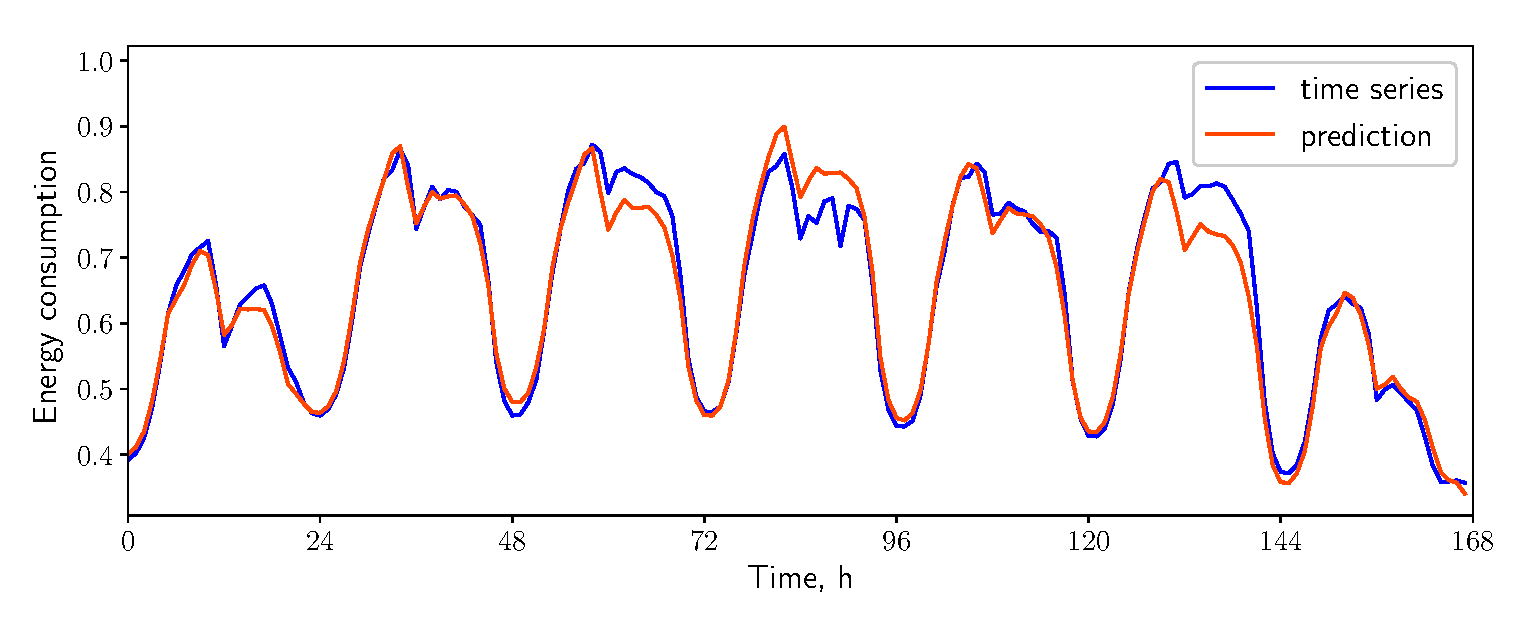
\includegraphics[width=0.8\linewidth]{figs/energy_prediction_pres.eps}
	\end{figure}
	\vspace{-0.5cm}
	\begin{figure}
		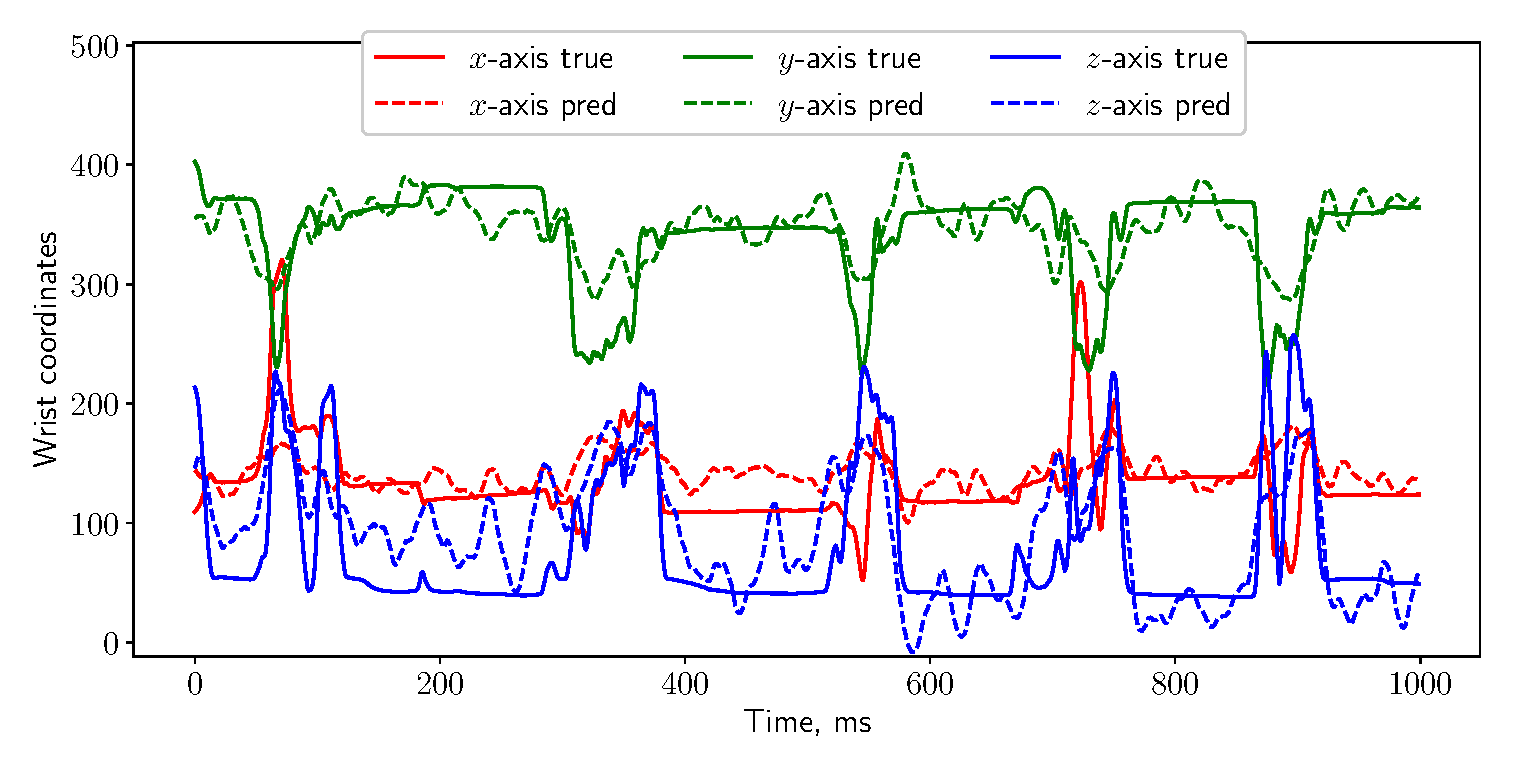
\includegraphics[width=0.8\linewidth]{figs/ecog_prediction_pres.eps}
	\end{figure}
\end{frame}
%--------------------------------------------------------------------------------
\end{document} 
